\documentclass[10pt,a4paper,twocolumn]{article}

% ── Geometry ──
\usepackage[margin=1.5cm,top=1.2cm,bottom=1.2cm,columnsep=0.6cm]{geometry}

% ── Fonts & encoding ──
\usepackage[T1]{fontenc}
\usepackage[utf8]{inputenc}
\usepackage{lmodern}
\usepackage{microtype}

% ── Math ──
\usepackage{amsmath,amssymb,bm}

% ── Tables ──
\usepackage{booktabs}
\usepackage{array}
\usepackage{tabularx}

% ── Colors & boxes ──
\usepackage[dvipsnames,svgnames]{xcolor}
\usepackage{tcolorbox}
\tcbuselibrary{breakable,skins}

% ── Code listings ──
\usepackage{listings}
\lstset{
  basicstyle=\ttfamily\scriptsize,
  breaklines=true,
  frame=none,
  backgroundcolor=\color{gray!8},
  xleftmargin=4pt,
  xrightmargin=4pt,
  aboveskip=4pt,
  belowskip=4pt,
  columns=fullflexible,
}

% ── Misc ──
\usepackage{enumitem}
\setlist{nosep,leftmargin=12pt}
\usepackage{titlesec}
\usepackage{fancyhdr}
\usepackage{tikz}
\usetikzlibrary{arrows.meta,positioning,calc}

% ── Section formatting ──
\titleformat{\section}
  {\large\bfseries\sffamily\color{MidnightBlue}}
  {\thesection}{0.5em}{}
  [\vspace{-2pt}\color{MidnightBlue}\hrule height 0.8pt\vspace{2pt}]

\titleformat{\subsection}
  {\normalsize\bfseries\sffamily\color{NavyBlue}}
  {\thesubsection}{0.5em}{}

\titleformat{\subsubsection}
  {\small\bfseries\sffamily\color{RoyalBlue}}
  {\thesubsubsection}{0.4em}{}

\titlespacing*{\section}{0pt}{8pt}{4pt}
\titlespacing*{\subsection}{0pt}{6pt}{2pt}
\titlespacing*{\subsubsection}{0pt}{4pt}{1pt}

% ── tcolorbox styles ──
\newtcolorbox{mathbox}[1][]{
  colback=blue!3,
  colframe=MidnightBlue!60,
  fonttitle=\small\bfseries\sffamily,
  boxrule=0.5pt,
  arc=2pt,
  left=4pt, right=4pt, top=3pt, bottom=3pt,
  before skip=4pt, after skip=4pt,
  #1
}

\newtcolorbox{promptbox}[1][]{
  colback=green!3,
  colframe=OliveGreen!60,
  fonttitle=\small\bfseries\sffamily,
  boxrule=0.5pt,
  arc=2pt,
  left=4pt, right=4pt, top=3pt, bottom=3pt,
  before skip=4pt, after skip=4pt,
  #1
}

\newtcolorbox{notebox}[1][]{
  colback=orange!4,
  colframe=BurntOrange!60,
  fonttitle=\small\bfseries\sffamily,
  boxrule=0.5pt,
  arc=2pt,
  left=4pt, right=4pt, top=3pt, bottom=3pt,
  before skip=4pt, after skip=4pt,
  #1
}

\newtcolorbox{algobox}[1][]{
  colback=violet!3,
  colframe=RoyalPurple!50,
  fonttitle=\small\bfseries\sffamily,
  boxrule=0.5pt,
  arc=2pt,
  left=4pt, right=4pt, top=3pt, bottom=3pt,
  before skip=4pt, after skip=4pt,
  #1
}

% ── Header/footer ──
\pagestyle{fancy}
\fancyhf{}
\renewcommand{\headrulewidth}{0.4pt}
\fancyhead[L]{\small\sffamily\color{gray} Semantic Branching --- Cheat Sheet}
\fancyhead[R]{\small\sffamily\color{gray} Sirjani \& Moore}
\fancyfoot[C]{\small\sffamily\color{gray} \thepage}

% ── Paragraph spacing ──
\setlength{\parindent}{0pt}
\setlength{\parskip}{3pt}

% ── Prevent overflow ──
\sloppy
\setlength{\emergencystretch}{1em}

% ══════════════════════════════════════════════════════════════
\begin{document}

\begin{center}
{\LARGE\bfseries\sffamily\color{MidnightBlue} Semantic Branching Cheat Sheet}\\[4pt]
{\normalsize\sffamily Semantic Entropy Clustering for Diverse Agentic Code Generation}\\[2pt]
{\small\color{gray}\sffamily Ramtin Sirjani \& Paul Moore --- Western University --- Gen AI 2026}
\end{center}

\vspace{4pt}
\begin{notebox}[title=Compute Budget]
Both baseline and branching are allowed \textbf{250 steps per trajectory}. The baseline runs a single greedy trajectory (250 steps total). Branching spawns up to $B{=}30$ trajectories, each with the same 250-step cap. Results: baseline 5/10, branching 4/10, \textbf{union 7/10} --- the methods are complementary.
\end{notebox}
\noindent\textcolor{MidnightBlue}{\rule{\columnwidth}{1pt}}
\vspace{2pt}

% ══════════════════════════════════════════════════════════════
\section{NLI Relevance Scoring (Search Phase)}

During the search phase the agent runs bash commands (\texttt{grep}, \texttt{find}, \texttt{cat}) to explore the repo. After \emph{each} step we score how relevant the finding is to the bug.

\subsection{Why Not Pure DeBERTa NLI?}

DeBERTa NLI is trained on \textbf{natural language} sentence pairs, not code-to-bug pairs.

\begin{small}
\begin{tabular}{@{}p{0.48\columnwidth}p{0.44\columnwidth}@{}}
\toprule
\textbf{Problem} & \textbf{Result} \\
\midrule
No shared context between code output and bug description & Entailment $\approx 0$ always \\
Too much shared context (copy-pasted keywords) & Entailment $\approx 1$ always \\
\bottomrule
\end{tabular}
\end{small}

\textbf{Solution}: use the LLM itself to bridge the domain gap via two cheap calls.

\subsection{Step 1 --- LLM Summarization}

Converts raw search output into a natural language sentence.

\begin{promptbox}[title=Summarization Prompt]
\scriptsize
An AI agent is debugging a software issue. It ran a search command and got this result. In one sentence, what did this search find and why might it be relevant?

\medskip
Agent's reasoning: \texttt{\{thought\}} {\color{gray}$\leftarrow$ 300 chars}

Search result (truncated): \texttt{\{observation\}} {\color{gray}$\leftarrow$ 500 chars}

One-sentence summary of what was found:
\end{promptbox}

\begin{small}
\texttt{temperature=0.0}, \texttt{max\_tokens=80}
\end{small}

\textbf{Output example}: {\small\emph{``Found the Permutation constructor in permutations.py which handles cycle notation input.''}}

\subsection{Step 2 --- LLM Relevance Rating}

\begin{promptbox}[title=Relevance Prompt]
\scriptsize
Rate how relevant this investigation finding is to the bug below.\\
Bug: \texttt{\{problem\_statement\}} {\color{gray}$\leftarrow$ 300 chars}\\
Finding: \texttt{\{finding\_summary\}} {\color{gray}$\leftarrow$ from Step 1}\\
Rate relevance from 0 (completely irrelevant) to 10 (directly identifies the bug).\\
Respond with ONLY a single number 0--10.
\end{promptbox}

\begin{small}
\texttt{temperature=0.0}, \texttt{max\_tokens=5}
\end{small}

\textbf{Post-processing}: regex extracts first integer $\to$ clamp to $[0,10]$ $\to$ divide by 10 $\to$ score~$\in [0,1]$.

\subsection{Why Not DeBERTa NLI for Relevance?}

We tested using DeBERTa entailment instead of LLM-as-judge (even with the LLM summary bridge). Results on sympy-16766:

\begin{scriptsize}
\begin{tabular}{@{}p{0.55\columnwidth}cc@{}}
\toprule
\textbf{Summary} & \textbf{NLI} & \textbf{LLM} \\
\midrule
``Found code generation utilities'' & 0.003 & 0.7 \\
``Found printing functionality files'' & 0.038 & 0.7 \\
``Found Python code printers module'' & 0.618 & 0.7 \\
``Found Indexed class docs'' & 0.005 & 0.7 \\
``mpmath missing, import failed'' & 0.017 & 0.3 \\
\bottomrule
\end{tabular}
\end{scriptsize}

\textbf{Why?} NLI measures \emph{logical entailment} (``does A imply B?''), not \emph{topical relevance}. ``Found Indexed class'' doesn't logically imply ``Indexed printing is broken'' --- but it's clearly relevant. NLI works for \textbf{clustering} (same-structure intent comparisons) but not for relevance scoring.

\subsection{Saturation Detection}

\begin{mathbox}[title=Saturation Rule]
\[
\text{consec\_low} \;\ge\; N_{\text{cap}} \;\Longrightarrow\; \textbf{Strategy Phase}
\]
A step is ``low relevance'' if $\text{score} \le \theta$\; (default $\theta = 0.5$).
\end{mathbox}


% ══════════════════════════════════════════════════════════════
\section{Generating 5 Diverse Strategies}

After search saturation: (1) build a \textbf{search report}, then (2) prompt for strategies.

\subsection{Search Report Prompt}

\begin{promptbox}[title=Search Report Prompt]
\scriptsize
An AI coding agent investigated a software bug. Below is its exploration history with the actual code it found.

Write a structured report with these sections:
\begin{enumerate}[nosep,leftmargin=10pt]
\item ROOT CAUSE: What is the bug and why?
\item RELEVANT CODE: Verbatim snippets with file/function/line.
\item FIX POINTS: Different places a fix could be applied.
\end{enumerate}

IMPORTANT: Include actual code from observations. Do NOT paraphrase.

Exploration history: \texttt{\{history\}} {\color{gray}$\leftarrow$ last 15 relevant steps, 8k chars}
\end{promptbox}

\begin{small}
\texttt{temperature=0.0}, \texttt{max\_tokens=1500}
\end{small}

\subsection{Strategy Proposal Prompt (Verbatim)}

\begin{promptbox}[title=Strategy Proposal Prompt]
\scriptsize
A software bug needs to be fixed. Here is the problem description and investigation findings.

\textbf{\#\# Problem}\\
\texttt{\{problem\_statement\}} {\color{gray}$\leftarrow$ 2000 chars}

\textbf{\#\# Investigation Findings}\\
\texttt{\{search\_report\}} {\color{gray}$\leftarrow$ 4000 chars}

\textbf{\#\# Task}\\
Propose exactly \texttt{\{n\}} FUNDAMENTALLY DIFFERENT code-level strategies to fix this bug.

CRITICAL RULES:
\begin{itemize}[nosep,leftmargin=8pt]
\item Each strategy MUST take a COMPLETELY DIFFERENT APPROACH
\item Each strategy MUST modify DIFFERENT lines, functions, or files
\item Each strategy MUST produce a structurally different patch
\item Do NOT propose strategies that all change the same line
\item Be SPECIFIC: name exact function, file, and line range
\item Describe the actual code transformation
\end{itemize}

Think about fundamentally different approaches:
\begin{itemize}[nosep,leftmargin=8pt]
\item Fix at different levels of the call stack
\item Fix in different files or modules
\item Use different mechanisms (validation vs normalization vs delegation)
\item Address different root causes
\end{itemize}

IMPORTANT: Before writing each strategy, explicitly state what makes it FUNDAMENTALLY DIFFERENT from all previous strategies.

Format: \texttt{STRATEGY 1: [file/function] --- [specific code change]}
\end{promptbox}

\begin{small}
$n=5$, \texttt{temperature=\textbf{1.0}} (high for diversity), \texttt{max\_tokens=1200}
\end{small}

\subsection{Iterative Rejection}

If $<5$ strategies parsed, a \textbf{second pass} explicitly rejects already-seen approaches:

\begin{promptbox}[title=Rejection Clause]
\scriptsize
Already Proposed Strategies (DO NOT repeat):\\
-- ALREADY PROPOSED: \texttt{\{strategy\_1\}}\\
-- ALREADY PROPOSED: \texttt{\{strategy\_2\}} \ldots

Propose \texttt{\{n\_more\}} NEW strategies targeting DIFFERENT code locations using DIFFERENT mechanisms.
\end{promptbox}


% ══════════════════════════════════════════════════════════════
\section{Bidirectional Entailment, Clustering \& Semantic Entropy}

\subsection{DeBERTa NLI Classification}

\subsubsection{Architecture (He et al.\ 2021)}

DeBERTa improves BERT with two ideas:

\begin{enumerate}[nosep,leftmargin=10pt]
\item \textbf{Disentangled attention} --- each token $i$ is represented by two vectors: content $\bm{H}_i$ and relative position $\bm{P}_{i|j}$. Attention decomposes into three terms:
\end{enumerate}

\begin{mathbox}[title=Disentangled Attention]
{\small
\[
A_{ij} = \underbrace{Q_i^c {K_j^c}^\top}_{\text{c2c}} + \underbrace{Q_i^c {K_{\delta}^r}^\top}_{\text{c2p}} + \underbrace{Q_{\delta}^r {K_j^c}^\top}_{\text{p2c}}
\]
}
{\scriptsize Scaled by $1/\sqrt{3d}$. p2p term dropped (no content info). $\delta{=}\delta(i,j)$ = relative distance, clamped to $[0, 2k)$.}
\end{mathbox}

\begin{enumerate}[nosep,leftmargin=10pt]\setcounter{enumi}{1}
\item \textbf{Enhanced mask decoder} --- absolute positions are incorporated \emph{after} all transformer layers (just before the softmax for MLM), not at the input like BERT. This lets the encoder use only relative positions.
\end{enumerate}

\subsubsection{Pre-training}

Masked language modeling (MLM) on large text corpora --- same objective as BERT/RoBERTa. DeBERTa-large: 24 layers, 1024 hidden, 16 heads.

\subsubsection{Fine-tuning on MNLI}

MNLI = 433k labeled (premise, hypothesis) pairs, each labeled \{entailment, neutral, contradiction\}. Fine-tuning adds a classification head on top:

\begin{scriptsize}
\begin{tabular}{@{}ll@{}}
\toprule
\textbf{Component} & \textbf{Detail} \\
\midrule
Encoder & DeBERTa $\to$ hidden states $[B, T, D]$ \\
ContextPooler & Dense + activation on \texttt{[CLS]} token \\
Dropout & Applied to pooled output \\
Classifier & Linear$(D, 3)$ $\to$ 3 logits \\
Loss & CrossEntropyLoss(logits, label) \\
\bottomrule
\end{tabular}
\end{scriptsize}

\subsubsection{Tokenization \& Input Format}

\textbf{Input}: (premise, hypothesis) pair $\to$ tokenized as:
\[
\texttt{[CLS]}\;\text{premise}\;\underbrace{\texttt{[SEP][SEP]}}_{\text{2 seps}}\;\text{hypothesis}\;\texttt{[SEP]}
\]

{\scriptsize \textbf{Why two \texttt{[SEP]}s?} DeBERTa V1 uses GPT-2 BPE vocab with BERT-style special tokens. HuggingFace's \texttt{DebertaTokenizer} places two \texttt{[SEP]} between pairs (verified empirically). All \texttt{token\_type\_ids} = 0 --- DeBERTa uses separator \emph{positions}, not type IDs, to distinguish premise from hypothesis.}

\subsubsection{Output}

\begin{mathbox}[title=Softmax to Probabilities]
\[
p_k = \frac{\exp(l_k)}{\sum_{j=0}^{2}\exp(l_j)} \qquad k \in \{0,1,2\}
\]
\end{mathbox}

\textbf{Output}: $\{p_0, p_1, p_2\}$ where $p_0 + p_1 + p_2 = 1$

\begin{small}
\begin{tabular}{@{}ccl@{}}
\toprule
\textbf{Index} & \textbf{Label} & \textbf{Meaning} \\
\midrule
0 & contradiction & Premise contradicts hypothesis \\
1 & neutral & Neither entails nor contradicts \\
2 & entailment & Premise implies hypothesis \\
\bottomrule
\end{tabular}
\end{small}

\subsection{Entailment Check}

Given threshold $\theta$ (default $= 0.5$):

\begin{mathbox}[title=One-Way Entailment]
\[
\textsc{ent}(A, B) = \bigl[\, p_2(A,\, B) > \theta \,\bigr]
\]
\smallskip
{\scriptsize where $p_2(A,B) = P(\text{entailment}\mid\text{prem}{=}A,\,\text{hyp}{=}B)$}
\end{mathbox}

\subsection{Bidirectional Entailment}

Two texts are \textbf{semantically equivalent} iff each entails the other:

\begin{mathbox}[title=Bidirectional Entailment]
\[
\textsc{bidir}(A,B) = \textsc{ent}(A,B) \;\wedge\; \textsc{ent}(B,A)
\]
\end{mathbox}

\begin{notebox}[title=Why bidirectional?]
\scriptsize
\begin{tabular}{@{}p{0.32\columnwidth}ccc@{}}
\toprule
\textbf{Pair} & \textbf{A$\to$B} & \textbf{B$\to$A} & \textbf{Bidir} \\
\midrule
``Fix constructor'' vs ``Modify code'' & \checkmark & $\times$ & \textbf{No} \\
``Remove dup check'' vs ``Delete redundant val.'' & \checkmark & \checkmark & \textbf{Yes} \\
``Add normalization'' vs ``Fix constructor'' & $\times$ & $\times$ & \textbf{No} \\
\bottomrule
\end{tabular}
\end{notebox}

\subsection{Clustering Algorithm}

\textbf{Algorithm 1} from Farquhar et al.\ 2024 / Kuhn et al.\ 2023.

\textbf{Context concatenation} (critical step from the paper):\\
Before any NLI comparison, prepend the problem context:
\[
\text{nli\_input}_i \;=\; \text{context} \;+\; \text{intent}_i
\]

\begin{algobox}[title=Greedy Sequential Clustering]
\begin{scriptsize}
\begin{tabbing}
\hspace{3mm}\=\hspace{3mm}\=\hspace{3mm}\=\kill
\textbf{In}: intents $[s_0, \ldots, s_{N-1}]$, context $C$, thr.\ $\theta$\\[2pt]
\textbf{Out}: clusters $\mathcal{K} = \{C_1, \ldots, C_K\}$\\[4pt]
$\mathcal{K} \leftarrow \emptyset$\\
\textbf{for} $i = 0$ \textbf{to} $N{-}1$:\\
\> $\text{assigned} \leftarrow \text{False}$\\
\> \textbf{for each} cluster $C_k \in \mathcal{K}$:\\
\>\> $r \leftarrow C_k.\text{rep}$\\
\>\> $\text{fwd} \leftarrow p_2(C{+}s_r,\; C{+}s_i)$\\
\>\> $\text{bwd} \leftarrow p_2(C{+}s_i,\; C{+}s_r)$\\
\>\> \textbf{if} fwd $> \theta$ \textbf{and} bwd $> \theta$:\\
\>\>\> add $i$ to $C_k$; assigned; \textbf{break}\\
\> \textbf{if not} assigned:\\
\>\> new cluster with rep $= i$
\end{tabbing}
\end{scriptsize}
\end{algobox}

\begin{scriptsize}
\begin{tabular}{@{}lp{0.52\columnwidth}@{}}
\toprule
\textbf{Property} & \textbf{Detail} \\
\midrule
Order-dep. & First intent $\to$ cluster rep \\
Greedy & Assigns to \emph{first} match \\
Single rep & Compares to cluster's first member \\
Complexity & $O(N {\times} K)$ NLI calls, $K \le N$ \\
\bottomrule
\end{tabular}
\end{scriptsize}

\subsection{Semantic Entropy}

\begin{mathbox}[title=Semantic Entropy (Discrete Variant)]
\[
H \;=\; -\sum_{k=1}^{K} p(c_k) \cdot \ln\bigl(p(c_k)\bigr)
\]
\vspace{-6pt}
\[
\text{where} \quad p(c_k) \;=\; \frac{|c_k|}{N}
\]
\end{mathbox}

\textbf{Every variable}:

\begin{scriptsize}
\begin{tabular}{@{}cp{0.65\columnwidth}@{}}
\toprule
\textbf{Sym.} & \textbf{Meaning} \\
\midrule
$H$ & Semantic entropy --- diversity in nats \\
$K$ & Number of semantic clusters \\
$k$ & Cluster index, $1$ to $K$ \\
$c_k$ & Cluster $k$ (set of candidate indices) \\
$|c_k|$ & Size of cluster $k$ \\
$N$ & Total candidates ($\sum_k |c_k|$) \\
$p(c_k)$ & Cluster probability $= |c_k|/N$ \\
$\ln$ & Natural log (base-$e$) \\
\bottomrule
\end{tabular}
\end{scriptsize}

\textbf{Bounds}:

\begin{small}
\begin{tabular}{@{}lcc@{}}
\toprule
\textbf{Scenario} & \textbf{Sizes} & $\bm{H}$ \\
\midrule
All in one cluster & $[5]$ & $0$ \\
Two equal groups & $[3,2]$ & $0.673$ \\
All singletons & $[1,1,1,1,1]$ & $\ln 5 \approx 1.609$ \\
\bottomrule
\end{tabular}
\end{small}

\textbf{Min}: $K{=}1 \Rightarrow p{=}1 \Rightarrow -1\cdot\ln 1 = 0$\\
\textbf{Max}: $K$ equal clusters $\Rightarrow H = \ln K$

\subsection{Branching Decision}

\begin{mathbox}[title=Branch Criterion]
\[
\text{branch} \;=\; \bigl[\; H > \tau \;\bigr] \qquad \text{default } \tau = 0.5
\]
\begin{itemize}[nosep,leftmargin=10pt]
\item $H > \tau$: diverse $\to$ \textbf{branch} --- each cluster spawns a trajectory
\item $H \le \tau$: converged $\to$ \textbf{no branch} --- take greedy action
\end{itemize}
\end{mathbox}

\subsection{Worked Example}

\textbf{5 strategies}, clustered with $\theta = 0.5$:

\begin{small}
\begin{tabular}{@{}cl@{}}
\toprule
& \textbf{Strategy} \\
\midrule
$s_0$ & Normalize overlapping cycles in constructor \\
$s_1$ & Raise ValueError when cycles share elements \\
$s_2$ & Canonicalize cycle input in from\_sequence \\
$s_3$ & Add validation in Permutation constructor \\
$s_4$ & Fix \_af\_new helper for overlapping cycles \\
\bottomrule
\end{tabular}
\end{small}

\textbf{Clustering trace}:

\begin{scriptsize}
\begin{tabular}{@{}cccp{0.35\columnwidth}@{}}
\toprule
$i$ & \textbf{fwd} & \textbf{bwd} & \textbf{Result} \\
\midrule
0 & -- & -- & New cluster $A{=}\{0\}$ \\
1 & .12 & -- & $<\theta$ $\to$ new $B{=}\{1\}$ \\
2 & .78 & .65 & Both $>\theta$ $\to$ $A{=}\{0,2\}$ \\
3 & .72 & .58 & Both $>\theta$ $\to$ $A{=}\{0,2,3\}$ \\
4 & .21 & -- & $<\theta$ for $s_0$, .15 for $s_1$ $\to$ new $C{=}\{4\}$ \\
\bottomrule
\end{tabular}
\end{scriptsize}

\textbf{Result}: 3 clusters, sizes $[3, 1, 1]$

\textbf{Entropy}:
\begin{align*}
p(A) &= \tfrac{3}{5} = 0.6, \quad p(B) = p(C) = \tfrac{1}{5} = 0.2 \\[4pt]
H &= -\bigl[0.6\ln(0.6) + 0.2\ln(0.2) + 0.2\ln(0.2)\bigr] \\
  &= -\bigl[0.6(-0.511) + 0.2(-1.609) + 0.2(-1.609)\bigr] \\
  &= -(-0.306 - 0.322 - 0.322) \\
  &= \mathbf{0.950}
\end{align*}

\textbf{Decision}: $0.950 > 0.5 = \tau$ $\;\Longrightarrow\;$ \textbf{BRANCH} into 3 trajectories.


% ══════════════════════════════════════════════════════════════
\section{SDLG --- Semantically Diverse Language Generation}

Aichberger et al.\ (2025). Generates diverse alternatives by gradient-based token attribution through DeBERTa, then substitution + LLM re-completion.

\begin{center}
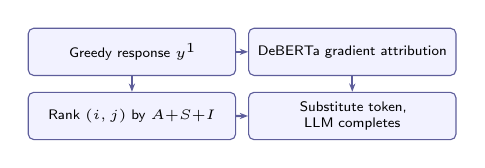
\begin{tikzpicture}[
  node distance=0.2cm,
  box/.style={rectangle, draw=MidnightBlue!70, fill=blue!5, rounded corners=2pt,
              font=\tiny\sffamily, text width=2.4cm, align=center, minimum height=0.6cm},
  arr/.style={-{Stealth[length=3pt]}, thick, MidnightBlue!70}
]
\node[box] (g) {Greedy response $y^1$};
\node[box, right=0.15cm of g] (a) {DeBERTa gradient attribution};
\node[box, below=0.2cm of g] (r) {Rank $(i,j)$ by $A{+}S{+}I$};
\node[box, below=0.2cm of a] (s) {Substitute token, LLM completes};
\draw[arr] (g) -- (a);
\draw[arr] (a) -- (s);
\draw[arr] (g) -- (r);
\draw[arr] (r) -- (s);
\end{tikzpicture}
\end{center}

\subsection{Step 0: Greedy Response}

Generate baseline at temp$\,{=}\,$0. Split into:

\begin{small}
\begin{tabular}{@{}ll@{}}
\toprule
\textbf{Part} & \textbf{Contents} \\
\midrule
THOUGHT & Natural language reasoning \\
CODE & Bash command in \texttt{```mswea\_bash\_command```} \\
\bottomrule
\end{tabular}
\end{small}

\subsection{Step 1: Attribution Score $A_i$}

\textbf{Goal}: Which tokens carry the most semantic weight?

\subsubsection{Setup --- Self-Entailment}

Feed text as \textbf{both} premise and hypothesis:

{\small
\[
\texttt{[CLS]}\;\underbrace{\text{text}}_{\text{prem.}}\;\texttt{[SEP]^2}\;\underbrace{\text{text}}_{\text{hyp.}}\;\texttt{[SEP]}
\]
}

\subsubsection{Loss --- Target Contradiction}

\begin{mathbox}[title=Contradiction Loss]
\[
\mathcal{L} = \text{CE}(\bm{l},\;\text{target}{=}0) = -\log\frac{\exp(l_0)}{\sum_k \exp(l_k)}
\]
\end{mathbox}

\textbf{Why contradiction?} The text trivially entails itself. The gradient of the contradiction loss reveals which tokens, if changed, would flip self-entailment to self-contradiction --- i.e., the tokens that carry the meaning.

\subsubsection{Backprop \& Attribution}

Backpropagate $\mathcal{L}$ through the embedding layer to get $\nabla_{\bm{z}_i}\mathcal{L}$ for each token $i$. Extract \textbf{hypothesis portion only}.

\begin{mathbox}[title=Attribution Score]
\[
A_i \;=\; \bigl\lVert\, \bm{z}_i \odot \nabla_{\!\bm{z}_i}\mathcal{L} \,\bigr\rVert_2
\]
\end{mathbox}

\textbf{Every symbol}:

\begin{small}
\begin{tabular}{@{}cp{0.62\columnwidth}c@{}}
\toprule
\textbf{Sym.} & \textbf{Meaning} & \textbf{Shape} \\
\midrule
$i$ & Token position in hypothesis & int \\
$\bm{z}_i$ & Embedding vector of token $i$ & $[D]$ \\
$D$ & Embedding dim (1024 for DeBERTa-large) & int \\
$\mathcal{L}$ & Contradiction loss & scalar \\
$\nabla_{\!\bm{z}_i}\mathcal{L}$ & Gradient of $\mathcal{L}$ w.r.t.\ $\bm{z}_i$ & $[D]$ \\
$\odot$ & Hadamard (element-wise) product & $[D]$ \\
$\lVert\cdot\rVert_2$ & L2 norm: $\sqrt{\sum_d (\cdot)^2}$ & scalar \\
$A_i$ & Attribution score for token $i$ & $\ge 0$ \\
\bottomrule
\end{tabular}
\end{small}

\textbf{Intuition for each piece}:

\begin{small}
\begin{tabular}{@{}lp{0.58\columnwidth}@{}}
\toprule
\textbf{Component} & \textbf{What it captures} \\
\midrule
$\bm{z}_i$ & Large embedding $=$ strong signal \\
$\nabla_{\!\bm{z}_i}\mathcal{L}$ & Large gradient $=$ loss sensitive to this token \\
$\bm{z}_i \odot \nabla$ & Both conditions simultaneously \\
$\lVert\cdot\rVert_2$ & Collapses $D$ dims to one scalar \\
\bottomrule
\end{tabular}
\end{small}

\textbf{Normalization}: $A_i \leftarrow A_i \,/\, \max_i(A_i)$ so $A_i \in [0,1]$.

\textbf{Word boundary filter}: Only word-initial BPE tokens (prefix \texttt{\.G} or \texttt{\_}) are candidates. Avoids sub-word fragments.

\subsection{Step 2: Substitution Score $S_{ij}$}

\textbf{Goal}: For position $i$, which replacement $j$ from the vocabulary shifts meaning most along the gradient?

\begin{mathbox}[title=Substitution Score]
\[
S_{ij} \;=\; \frac{(\bm{z}_i - \bm{z}_j) \;\cdot\; \nabla_{\!\bm{z}_i}\mathcal{L}}{\lVert \bm{z}_i - \bm{z}_j \rVert_2 \;\cdot\; \lVert \nabla_{\!\bm{z}_i}\mathcal{L} \rVert_2}
\]
\end{mathbox}

\textbf{Every symbol}:

\begin{scriptsize}
\begin{tabular}{@{}cp{0.62\columnwidth}@{}}
\toprule
\textbf{Sym.} & \textbf{Meaning} \\
\midrule
$\bm{z}_i$ & Embedding of original token at pos $i$ \\
$\bm{z}_j$ & Embedding of candidate replacement $j$ \\
$\bm{z}_i{-}\bm{z}_j$ & How much the embedding changes \\
$\nabla\mathcal{L}$ & Direction increasing contradiction \\
$\cdot$ & Dot product \\
$S_{ij}$ & Cosine sim.\ of change vs gradient \\
\bottomrule
\end{tabular}
\end{scriptsize}

\textbf{Interpretation}:

\begin{scriptsize}
\begin{tabular}{@{}cp{0.65\columnwidth}@{}}
\toprule
$S_{ij}$ & \textbf{Meaning} \\
\midrule
${\approx}{+}1$ & Moves along gradient $\to$ max meaning change \\
${\approx}\;0$ & Orthogonal $\to$ no semantic shift \\
${\approx}{-}1$ & Against gradient $\to$ reinforces original \\
\bottomrule
\end{tabular}
\end{scriptsize}

Computed \textbf{server-side} over the full vocabulary ($V \approx 128$k):

\begin{lstlisting}[language=Python]
diff = z_i.unsqueeze(0) - emb_matrix   # [V, D]
diff_norms = diff.norm(dim=-1)          # [V]
s_ij = (diff @ grad_i) / (diff_norms * grad_norm)
\end{lstlisting}

Top-$K$ ($K{=}20$) replacements selected. Self-substitution excluded.

\subsection{Step 3: Importance Score $I_{ij}$}

\textbf{Goal}: Is the substitute plausible under the LLM?

\begin{mathbox}[title=Importance Score]
\[
I_{ij} \;=\; p\bigl(v_j \;\big|\; y_{<i},\; x,\; w\bigr)
\]
\end{mathbox}

\begin{small}
\begin{tabular}{@{}cl@{}}
\toprule
\textbf{Symbol} & \textbf{Meaning} \\
\midrule
$v_j$ & Candidate replacement token \\
$y_{<i}$ & All text before position $i$ \\
$x$ & Full conversation context (history) \\
$w$ & LLM weights (Qwen3-Coder-30B) \\
$p(\cdot)$ & LLM's next-token distribution \\
\bottomrule
\end{tabular}
\end{small}

\textbf{Computed via vLLM}: send prefix to \texttt{/v1/completions} with \texttt{logprobs=20}, convert: $I_{ij} = \exp(\text{logprob}_j)$.

\begin{notebox}[title=Why I\textsubscript{ij} matters]
\scriptsize
Without $I_{ij}$, SDLG might substitute ``remove'' $\to$ ``xylophone'' (high $S_{ij}$ because embeddings are far apart, but nonsensical). $I_{ij}$ filters for tokens the LLM would actually generate.
\end{notebox}

\subsection{Step 4: Combined Ranking}

\begin{mathbox}[title=Combined Score]
\[
\text{Combined}_{ij} \;=\; \frac{A_i \;+\; S_{ij} \;+\; I_{ij}}{3}
\]
\end{mathbox}

\begin{scriptsize}
\begin{tabular}{@{}ccp{0.32\columnwidth}l@{}}
\toprule
 & \textbf{Range} & \textbf{Measures} & \textbf{Source} \\
\midrule
$A_i$ & $[0,1]$ & Position importance & DeBERTa $\nabla$ \\
$S_{ij}$ & $[-1,1]$ & Meaning shift & emb+$\nabla$ \\
$I_{ij}$ & $[0,1]$ & LLM plausibility & vLLM \\
\bottomrule
\end{tabular}
\end{scriptsize}

All $(i, j)$ pairs sorted by Combined$_{ij}$ descending.

\subsection{Step 5: Prefix Truncation \& Completion}

\subsubsection{THOUGHT-Level (Strategic Diversity)}

Changes the \emph{reasoning}, causing a different fix approach:

\begin{algobox}[title=Thought Substitution]
\begin{enumerate}[nosep,leftmargin=10pt]
\item Find original token in thought text
\item Replace with substitute
\item \textbf{Truncate everything after} substitution point
\item Send truncated thought as \texttt{assistant} message prefix
\item LLM regenerates rest of reasoning \textbf{AND} code
\end{enumerate}
\end{algobox}

\textbf{Example}:
\begin{small}
\begin{itemize}[nosep]
\item Greedy: ``I should \textbf{remove} the duplicate check\ldots''
\item Substitute: ``remove'' $\to$ ``compose''
\item Prefix: ``I should compose''
\item LLM completes: ``\ldots the cycles before validation\ldots'' + \emph{new code}
\end{itemize}
\end{small}

\subsubsection{CODE-Level (Tactical Diversity)}

Keeps reasoning fixed, diversifies the implementation:

\begin{algobox}[title=Code Substitution]
\begin{enumerate}[nosep,leftmargin=10pt]
\item Keep thought text \textbf{unchanged}
\item Find original token in code block
\item Replace with substitute, truncate
\item LLM completes the code from there
\item Result: same reasoning, different patch
\end{enumerate}
\end{algobox}

\subsubsection{Budget Split}

For $N$ total candidates (default $N{=}5$):

\begin{small}
\begin{tabular}{@{}ll@{}}
\toprule
\textbf{Source} & \textbf{Count} \\
\midrule
Greedy response (always kept) & 1 \\
THOUGHT-level SDLG & $\lceil(N{-}1)/2\rceil = 2$ \\
CODE-level SDLG & $\lfloor(N{-}1)/2\rfloor = 2$ \\
\bottomrule
\end{tabular}
\end{small}

\subsection{Fallback}

If SDLG produces zero alternatives $\to$ \textbf{temperature sampling} at $T{=}0.7$.

\end{document}
